现在不加证明地陈述 Lemma~\ref{lem:flat-boundary-local-regularity} 的 ``高阶\textquotesingle\textquotesingle\ 版本.

\begin{Lemma}
\label{lem:higher-order-flat-boundary-regularity}
设 Lemma~\ref{lem:flat-boundary-local-regularity} 的假设成立. 再假设系数满足 $a_{ij}\in W^{k+1,\infty}(D^+)$, $b_i,c\in W^{k,\infty}(D^+)$, 且 $f\in H^k(D^+)$. 则 $u\in H^{k+2}(Q^+)$, 且存在依赖于 $R$ 的常数 $C$, 使得
\begin{equation}\label{eq:higher-order-flat-boundary-local-regularity-estimate}
\|u\|_{H^{k+2}(Q^+)}\leq C(\|f\|_{H^k(D^+)}+\|u\|_{H^1(D^+)}).
\end{equation}

\end{Lemma}

为证明 Theorem~\ref{thm:global-boundary-regularity}, 必须考虑一般区域 $\Omega$. 当然, 由于 Lemma~\ref{lem:flat-boundary-local-regularity} 的全部证明都在半空间上进行, 下一步需要 ``展平\textquotesingle\textquotesingle\ $\Omega$ 的边界. 由于 $\partial\Omega$ 是 $C^2$ 曲面, 对每个 $\overline{\bm{x}}\in\partial\Omega$, 都存在 $R>0$ 和 $C^2(\mathbb{R}^{n-1})$ 函数 $\psi$, 使得 (必要时重新编号并调整坐标方向后)
\begin{equation}\label{eq:boundary-local-graph-coordinate-description}
\partial\Omega\cap B_R(\overline{\bm{x}})=\{\bm{x}\in B_R(\overline{\bm{x}})\mid x_n=\psi(x_1,x_2,\ldots,x_{n-1})\},
\end{equation}

\begin{equation}\label{eq:boundary-local-domain-above-graph-description}
\Omega\cap B_R(\overline{\bm{x}})=\{\bm{x}\in B_R(\overline{\bm{x}})\mid x_n>\psi(x_1,x_2,\ldots,x_{n-1})\};
\end{equation}
此外, 由\[\begin{aligned}
y_i&:=x_i-\overline x_i,\quad i=1,\ldots,n-1,\\
y_n&:=x_n-\psi(x_1,\ldots,x_{n-1})
\end{aligned}\]定义的映射
\begin{equation}\label{eq:boundary-straightening-forward-coordinate-map}
B_R(\overline{\bm{x}})\ni\bm{x}\mapsto\bm{y}=\Psi(\bm{x})\in\mathbb{R}^n
\end{equation}
是一一的. 定义 $\overline\Phi:=\Psi^{-1}$. 注意 $\Phi$ 是一个 $C^2$ 函数, 将集合 $\Omega^{\prime}:=\Omega\cap B_R(\overline{\bm{x}})$ (在所谓的 $\bm{x}$ 空间中) 变换为 ($\bm{y}$ 空间的) 半空间 $y_n>0$ 中的集合 $\Omega^{\prime\prime}$. 还应注意, 点 $\overline{\bm{x}}$ 被映到 $\bm{y}$ 空间的原点 (参见 Figure~\ref{fig:boundary-straightening-original}).

\begin{figure}[H]
\centering
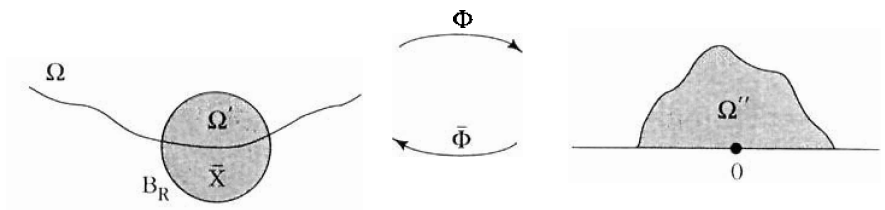
\includegraphics[width=.78\linewidth]{figures/chapter-09-boundary-straightening-original.png}
\caption{展平边界.}\label{fig:boundary-straightening-original}
\end{figure}
